% Chapter Template

\chapter{Experiments and results} % Main chapter title

\label{Chapter5} % Change X to a consecutive number; for referencing this chapter elsewhere, use \ref{ChapterX}

\lhead{Chapter 5. \emph{Experiments and results}} % Change X to a consecutive number; this is for the header on each page - perhaps a shortened title

After discussing how crawl.js works we want to run some experiments. We decided to test crawl.js in a closed environment. Crawling the public internet requires a good supervision and the required work to do that is simply out of scope for this thesis. All experiments were done on the opennebula cluster hosted at the university of neuchatel.
\\
First we describe our \emph{setup} and afterwards we discuss the different experiments we ran on it. \emph{Experiment 1} focuses on verifying basic properties of crawl.js (e.g. scaling). In \emph{Experiment 2 \& 3} we introduce latency and compare two different \emph{mapper}~\ref{mapper} approaches. A simple (random,hash) URL to worker assignment and a 2-level assignment.


%Furthermore we want to verify the \emph{closeness}~\ref{closeness} aspect of crawl.js. Crawl.js is configurable in such a way that sites that are \emph{close} (in terms of latency) to a worker are assigned to them. In order to do that we will add virtual latency to some of the sites and compare two different mapper~\ref{mapper} implementations:
%\begin{itemize}
%\item Simple - the whole URL is hashed. Therefore the site to worker assignment is random.
%\item 2-level - the host part of the URL identifies the group of workers. (a group that is \emph{close}). The remaining part of the URL determines the worker inside the group.
%\end{itemize}

\section{Setup}
To do our experiments we had to setup the following types of VM in the cluster:
\begin{itemize}
\item www - static wikipedia snapshots.
\item redis - remote queues.
\item workers - crawls pages from \emph{www} and updates remote queues in \emph{redis}.
\end{itemize}

To setup and manage (workers) the VMs efficiently we wrote some basic bash scripts. It allowed us to deploy different worker configurations easily and perform basic operations on the workers such as start and stop. Having those scripts saved us a lot of time throughout the different experiments we ran. You find all scripts used throughout our experiments in the crawl.js git repository. In Figure~\ref{test_setup} is an overview of all the VMs used during the experiments.

\begin{figure}[h]
\centering
  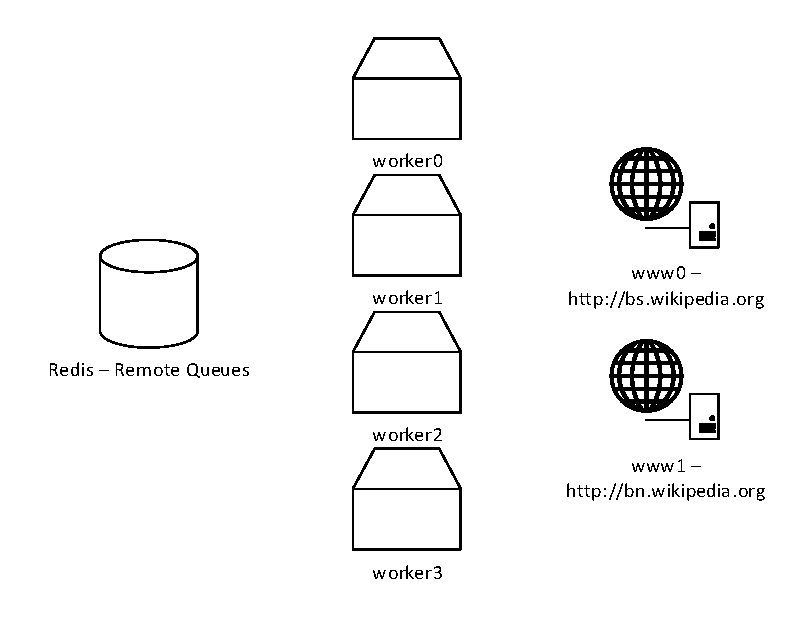
\includegraphics[width=1.0\textwidth]{Figures/experiments_setup.pdf}
\caption{Crawl.js - Test setup overview}
\label{test_setup}
\end{figure}

\subsection{www - wikipedia snapshots}
In order to have realistic sites to crawl we decided to setup wikipedia html dumps. Unfortunately their dumper stopped back in 2008 and therefore the snapshots are pretty old. But for our use case it is good enough. Almost. Back then, the different wikipedia languages were located in different subdirectories. All on the same server. But we need links pointing to different servers to be able to add latency to some of the sites and experiment with the \emph{closeness} aspect of crawl.js. Therefore we wrote an xsl transformation script to change all language links from /de/index.html to de.wikipedia.org/index.html.


Additionally we encountered a serious performance problem during our first tests. The random read performance in our VM was about 200 IOPS (tested with fio). Therefore the web server (nginx) could not deliver pages fast enough and represented the bottleneck in our setup. In order to circumvent this unwanted side effect we put our html dumps on a ramfs.

\begin{itemize}
  \item CPU: 1, VCPU: 1
  \item RAM: 2048M
\end{itemize}

\subsection{redis - Remote queues}
This setup was pretty simple. Just a single redis server instance running. Because all the URLs have to fit in memory, setting up a redis cluster to share the key space on different servers is inevitable as soon the number of URLs becomes too big. In our simple/small setup this was not needed. During our experiments we encountered 217'690 URLs which represents 82M of data inside the redis server (redis info command).

\begin{itemize}
  \item CPU: 1, VCPU: 1
  \item RAM: 3072M
\end{itemize}

\subsection{worker - Crawl.js worker instance}
The worker VM hosts our developed crawler (crawl.js instance). Setting it up was straight forward. First we thought that we could host more than one crawler instance (using multiple cpus) but we achieved better results with one crawler per worker. This 1:1 worker to crawler relation made the management easier too.

\begin{itemize}
  \item CPU: 1, VCPU: 1
  \item RAM: 1024M
\end{itemize}

\section{Experiment 1 (basic properties, scaling)}

The goal of our first experiment was to verify the following basic properties of crawl.js.

\begin{itemize}
\item The crawl stops
\item Adding more workers reduces the crawl duration (1, 2 \& 4 workers)
\item All pages are found (starting with a single seed URL)
\end{itemize}

 All tests (1, 2 and 4 workers) started with the same seed URL (http://bn.wikipedia.org) and as shown in Figure~\ref{plot:exp_001} the first results verified both properties: \emph{The crawl stops} and \emph{Adding more workers reduces the crawl duration}. The scaling behaviour actually exceeded our expectations as it was almost linear. The communication overhead needed to perform a crawl with more than 1 worker was minimal. A possible explanation for this overhead is worker idle times. Because every worker flushes the newly found URLs only once every 10 seconds (configurable), other workers could ran out of work and be forced to wait (and re ask later). Verifying this assumption would require an additional experiment. Basically exactly the same experiment but starting with many seed URLs (those found during this experiment for example). We are pretty sure that with a big seed list idling would not happen or at least be shorter.
\newline
\newline
For the last property \emph{All pages are found} wikipedia provides a downloadable text file containing all article URLs. Using this file we were able to import the expected URLs into redis (set datastructure). Afterwards we took the difference (redis diff) between the two sets 'urls:expected' and 'urls:crawled'. Unfortunately the resulting set was not empty. It had 23'338 URLs. That number seemed us pretty huge, thats about 16\% of all articles. Did we miss that many URLs? We decided to have a closer look at some randomly picked articles to check what we actually missed. We discovered quickly that most of these 'missed' articles redirected (alias) to other articles we did crawl (13'391 redirect articles). Because articles never reference articles through an alias, crawl.js did not discover those 'redirect-articles' (as we follow references,<a> tags). This still leaves us with 9'947 (7\%) of potentially missed articles. Again we randomly picked some of the remaining articles and discovered that none of them were referenced by other articles (using grep -r). Of course we did not check for references to all remaining articles but 7\% of orphaned articles~\footnote{\url{http://en.wikipedia.org/wiki/Wikipedia:WikiProject_Orphanage}} seemed us realistic and therefore the verification of this property good enough to proceed with our experiments.
\newline
\newline
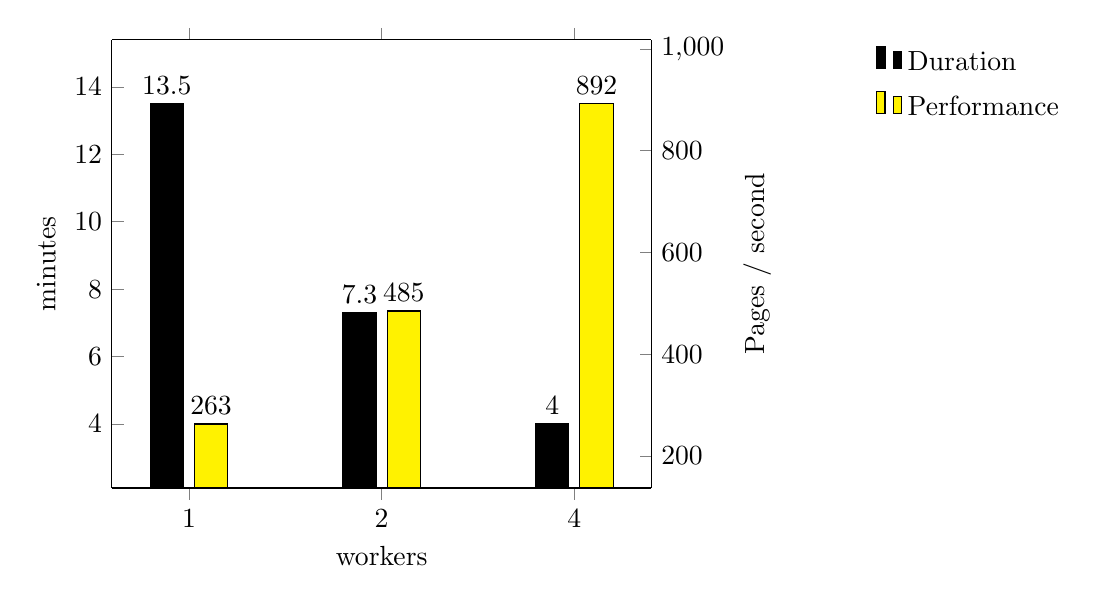
\begin{tikzpicture} 
  \begin{axis}[
    ybar,
    bar width=12pt,
    bar shift=-8pt,
    axis y line*=left,
    enlargelimits=0.2,
    xlabel={workers},
    xlabel near ticks,
    ylabel={minutes},
    ylabel near ticks,
    xtick=data,
    symbolic x coords={1,2,4},
    legend style={at={(1.4,1)}, anchor=north west, draw=none},
    nodes near coords,
    nodes near coords align={vertical},
    ]
    \addplot[fill=black]
      coordinates {(1,13.5) (2,7.3) (4,4.0)};
    \legend{Duration}
  \end{axis}
  \begin{axis}[
    ybar,
    bar width=12pt,
    bar shift=8pt,
    axis y line*=right,
    hide x axis,
    enlargelimits=0.2,
    ylabel={Pages / second},
    ylabel near ticks,
    symbolic x coords={1,2,4},
    legend style={at={(1.4,0.9)},anchor=north west, draw=none},
    nodes near coords,
    nodes near coords align={vertical},
    ]
    \addplot[fill=yellow]
      coordinates {(1,263) (2,485) (4,892)};
  \legend{Performance}
  \end{axis}
\label{plot:exp_001}
\end{tikzpicture}

\subsection{Configuration}

Here is an overview of the configuration we used.

\begin{itemize}
  \item Mapper: simple (random URL to worker assignment)
  \item Sites: http://bn.wikipedia.org, http://bs.wikipedia.org (142'082 articles)
  \item Site latencies: None
\end{itemize}

\section{Experiment 2}

\section{Experiment 3}
